\section{Software: from firmware to UI}\label{sec:software}

\begin{figure}[H]\centering
\begin{tikzpicture}[
  box/.style={draw, rounded corners=2pt, align=center, font=\small, inner sep=4pt},
  arr/.style={{Stealth}-{Stealth}, thick},
  lab/.style={font=\scriptsize, align=center}]
  \node[box, fill=blue!5, text width=2.6cm] (ui) at (0,0.75) {Browser UI\\\scriptsize BumpemUI/web};
  \node[box, fill=blue!5, text width=2.6cm] (other) at (0,-0.75) {MATLAB, scripts,\\\scriptsize curl, future apps};
  \node[box, fill=green!6, text width=3.1cm, minimum height=2.8cm] (srv) at (4.9,0) {\textbf{bumpem serve}\\\scriptsize Python, FastAPI\\\scriptsize bumpem/server.py\\[3pt]\scriptsize owns the serial port\\\scriptsize settings, recording};
  \node[box, fill=orange!8, text width=3.1cm, minimum height=2.8cm] (fw) at (10.0,0) {\textbf{Teensy 4.1}\\\scriptsize firmware v1\\\scriptsize firmware/src/main.ino\\[3pt]\scriptsize 10\,ms force loop\\\scriptsize limits, e-stop};
  \node[box, text width=2.0cm] (hw) at (14.1,0) {DAC, ESCONs, amplifiers};
  \draw[arr] (ui.east) -- node[lab, above]{HTTP + WS} (ui.east -| srv.west);
  \draw[arr] (other.east) -- node[lab, above]{HTTP} (other.east -| srv.west);
  \draw[arr] (srv) -- node[lab, above]{USB serial} node[lab, below]{protocol v1} (fw);
  \draw[arr] (fw) -- (hw);
  \node[lab, below=0.15cm of srv] {contract: docs/API.md};
  \node[lab, below=0.15cm of fw] {contract: docs/PROTOCOL.md};
\end{tikzpicture}
\caption{Software layers. Each arrow has one written contract; change the contract first, then the code
on both sides.}
\end{figure}

Why this split (\file{docs/DECISIONS.md} D6, D9, D10):
\begin{itemize}
\item The \textbf{Teensy} does all real-time work and all safety limits (force clamp, over-force fault,
e-stop, watchdog). It knows channels, forces and times, nothing about angles or gait.
\item The \textbf{server} is the only program that opens the serial port, so the stop command can never be
blocked by another program (the old MATLAB + serial monitor setup had exactly that problem). It turns
angles into per-module forces and will schedule gait-triggered perturbations.
\item The \textbf{UI} is replaceable. It uses only the HTTP API, never the Python code. Closing the browser
changes nothing on the board.
\item Everything runs without hardware: \file{bumpem/sim.py} is a simulated board that speaks the same
protocol. Use it first for every change.
\end{itemize}

\subsection{Firmware v1}\label{sec:firmware}
Built and flashed with PlatformIO: \file{scripts/flash.sh} (settings and pinned library versions in
\file{firmware/platformio.ini}). The original thesis code stays untouched in \file{legacy/};
\file{scripts/flash.sh} \cmd{legacy} builds it as a reference. Confirm with the project lead before flashing.

\paragraph{States.} \cmd{DISARMED} at boot (drivers off, no tension) $\rightarrow$ \cmd{ARM} ramps 0 to
baseline over \cmd{arm\_ms} $\rightarrow$ \cmd{ARMED} (holding baseline, pulses allowed) $\rightarrow$
\cmd{RELEASE} ramps to 0, drivers off. Any state $\rightarrow$ \cmd{ESTOP} (drivers off, DAC 0 at once;
recover with \cmd{ARM}). Measured force above \cmd{fault\_n} for \cmd{fault\_ms} $\rightarrow$ \cmd{FAULT}.

\paragraph{Control law} (per enabled module, every \cmd{loop\_ms}):
\[
i_\mathrm{des} = k_p\,(F_\mathrm{target}-F) - k_d\,\frac{\Delta F}{\Delta t}
  + k_\mathrm{ff}\,F_\mathrm{target}\,\frac{r_c}{k_t},\qquad
\mathrm{DAC} = \mathrm{clamp}\!\left(\frac{i_\mathrm{des}}{i_\mathrm{full}},0,1\right)\cdot 4095
\]
With $k_p = k_d = 0$ the loop is open: the motor gets a current proportional to the target and the force
sensor is ignored. ``Armed'' does not mean ``closed loop''; the gains decide.

\begin{table}[H]\centering\small
\begin{tabularx}{\linewidth}{lllX}
\toprule
Parameter & Default & Used on 6 Oct & Meaning \\
\midrule
\cmd{kp\_track}, \cmd{kd\_track} & 0.24, 3.5 & default & PD gains while holding baseline \\
\cmd{kp\_pulse}, \cmd{kd\_pulse} & 0.24, 3.5 & default & PD gains during a pulse \\
\cmd{kff} & 7.5 & 2 & feedforward multiplier (Stanford: 1) \\
\cmd{rc}, \cmd{kt} & 0.01905, 0.1524 & default & drum radius (m), torque constant \\
\cmd{i\_full} & 30 & default & current at DAC full scale (real: 9.9\,A, Sect.~2) \\
\cmd{baseline\_n} & 5 & 2 & holding tension, N \\
\cmd{fmax\_n} & 200 & 40 & largest allowed target, N (hard ceiling 200) \\
\cmd{fault\_n}, \cmd{fault\_ms} & 195, 20 & default & over-force fault \\
\cmd{filter\_hz}, \cmd{d\_window} & 0, 1 & default & force filter (0 = off), derivative window \\
\cmd{ch\_A}\ldots\cmd{ch\_D} & 1,1,1,0 & set by server & module enabled \\
\cmd{gain\_X}, \cmd{offset\_X} & 1, 0 & offsets zeroed & per-sensor calibration \\
\cmd{wd\_ms} & 0 & 1000 (server) & watchdog: no message for this long $\rightarrow$ abort pulse \\
\bottomrule
\end{tabularx}
\caption{Main parameters (full list in \file{docs/PROTOCOL.md}). They live in the Teensy's RAM: a replug
resets them, which is why the server reapplies saved settings.}
\end{table}

\paragraph{Serial protocol.} One text line per message. Host $\rightarrow$ board: \cmd{INFO}, \cmd{GET},
\cmd{SET name value}, \cmd{ARM}, \cmd{PULSE id delay rise dur fall aA aB aC aD}, \cmd{ABORT},
\cmd{RELEASE}, \cmd{ESTOP}, \cmd{CLEAR}, \cmd{STATS}, \cmd{PING}. Every command gets one \cmd{A,OK} or
\cmd{A,ERR} line. Board $\rightarrow$ host: telemetry \cmd{T,ms,state,pulse\_id,} then target, measured and
DAC value for A--D, 100 lines/s; events \cmd{E,...} (pulse start/end, state changes, faults).
Pulse amplitudes are relative to baseline; duration runs from start to end including both ramps.

\subsection{Python package and server}
Install once (conda env \cmd{BumpemHome} on the lab Mac):
\begin{lstlisting}
cd BumpemServer
pip install -e ".[server,dev]"
pytest                      # 52 tests, no hardware needed
\end{lstlisting}

\begin{table}[H]\centering\small
\begin{tabularx}{\linewidth}{lX}
\toprule
Module & Role \\
\midrule
\file{protocol.py} & message types and parser; mirrors \file{docs/PROTOCOL.md} \\
\file{device.py} & \cmd{Board} client: request/ack, telemetry, e-stop, over a serial link or the simulator \\
\file{sim.py} & simulated board speaking protocol v1 \\
\file{server.py} & HTTP/WebSocket server (FastAPI) \\
\file{geometry.py} & angle $\rightarrow$ per-module amplitudes \\
\file{datalog.py} & CSV recordings \\
\file{cli.py} & the \cmd{bumpem} command \\
\file{gait.py}, \file{experiment.py}, \file{recovery.py}, \file{vicon.py} & foot-strike detection (port of the MATLAB script, not yet validated), trial sequences, balance-recovery hook, Vicon client (stub) \\
\bottomrule
\end{tabularx}
\end{table}

\paragraph{Starting the server.}
\begin{lstlisting}
bumpem serve --board /dev/cu.usbmodem169222501 --modules ACD   # production (default)
bumpem serve --testing --board /dev/cu.usbmodem169222501       # one test pull per motor
bumpem serve --board sim                                        # no hardware
\end{lstlisting}
Then open \url{http://127.0.0.1:8000/} (UI) or \url{http://127.0.0.1:8000/docs} (try every endpoint).
Options: \cmd{--modules} (mounted modules; use \cmd{ABCD} once tower B runs), \cmd{--settings}
(default \file{settings.json}), \cmd{--log-dir} (default \file{Logs/}), \cmd{--wd-ms} (board watchdog,
default 1000), \cmd{--host} (default 127.0.0.1, this PC only), \cmd{--ui}.

\begin{table}[H]\centering\small
\begin{tabularx}{\linewidth}{llX}
\toprule
Method & Path (\cmd{/api/v1/...}) & Does \\
\midrule
GET/POST & \cmd{info}, \cmd{ports}, \cmd{connect}, \cmd{disconnect} & connection (\cmd{\{"port":"sim"\}} for the simulator) \\
GET/PATCH & \cmd{status}, \cmd{params} & board state, read/change parameters \\
POST & \cmd{arm}, \cmd{release}, \cmd{abort}, \cmd{estop}, \cmd{clear} & state changes \\
POST & \cmd{pulse} & one pulse, amplitudes per module \\
POST & \cmd{perturbation} & one pulse by angle + resultant amplitude \\
GET & \cmd{geometry} & module angles, reachable directions \\
GET/POST/DELETE & \cmd{settings} & saved parameters, reapplied at every connect \\
GET/POST & \cmd{log}, \cmd{log/start}, \cmd{log/stop} & recording to \file{Logs/force_*.csv} + \file{events_*.csv} \\
POST & \cmd{test/pull} & testing mode only: one open-loop pull on one module \\
WS & \cmd{stream} & live telemetry (30\,Hz for display) and events; accepts \cmd{\{"type":"estop"\}} \\
\bottomrule
\end{tabularx}
\caption{Implemented endpoints (\file{docs/API.md}). Errors come back as
\cmd{\{"error":\{"code":...,"message":...\}\}}; \cmd{board\_lost} (503) means the USB link is gone: replug,
then Disconnect and Connect.}
\end{table}

Example from MATLAB:
\begin{lstlisting}
opts = weboptions('MediaType', 'application/json');
webwrite('http://127.0.0.1:8000/api/v1/perturbation', struct('angle_deg', 135, ...
         'amplitude_n', 20, 'phase1_ms', 50, 'dur_ms', 400, 'phase2_ms', 50), opts);
\end{lstlisting}

\subsection{Browser UI}
Plain HTML, CSS and JavaScript in \file{BumpemUI/web}, no build step, works offline. The server serves it
at \cmd{/ui/}. Two pages, matching the server mode:
\begin{itemize}
\item \textbf{Testing} (\file{testing.html}, \cmd{--testing}): per motor a force and a duration, then
\emph{Pull}. No arming, no constant tension. Use it to check that each rope moves after any wiring change.
\item \textbf{Production} (\file{index.html}, default): Connect, Arm, Release, Clear; direction dial
(grey = no mounted module can pull that way); perturbation amplitude, ramps, duration, delay with a profile
preview; board settings (baseline, max force, feedforward gain, channels); \emph{Zero sensors} (2\,s mean
$\rightarrow$ offsets, ropes slack); \emph{Save as default}; \emph{Record} with a label; live force plot
(measured solid, target dashed); gait-phase picker (disabled until the server has PTO).
\end{itemize}
\textbf{STOP} (red button or the Esc key) is on every page. STOP and Release drop rope tension: stop the
treadmill first unless it is an emergency.

\begin{figure}[H]\centering
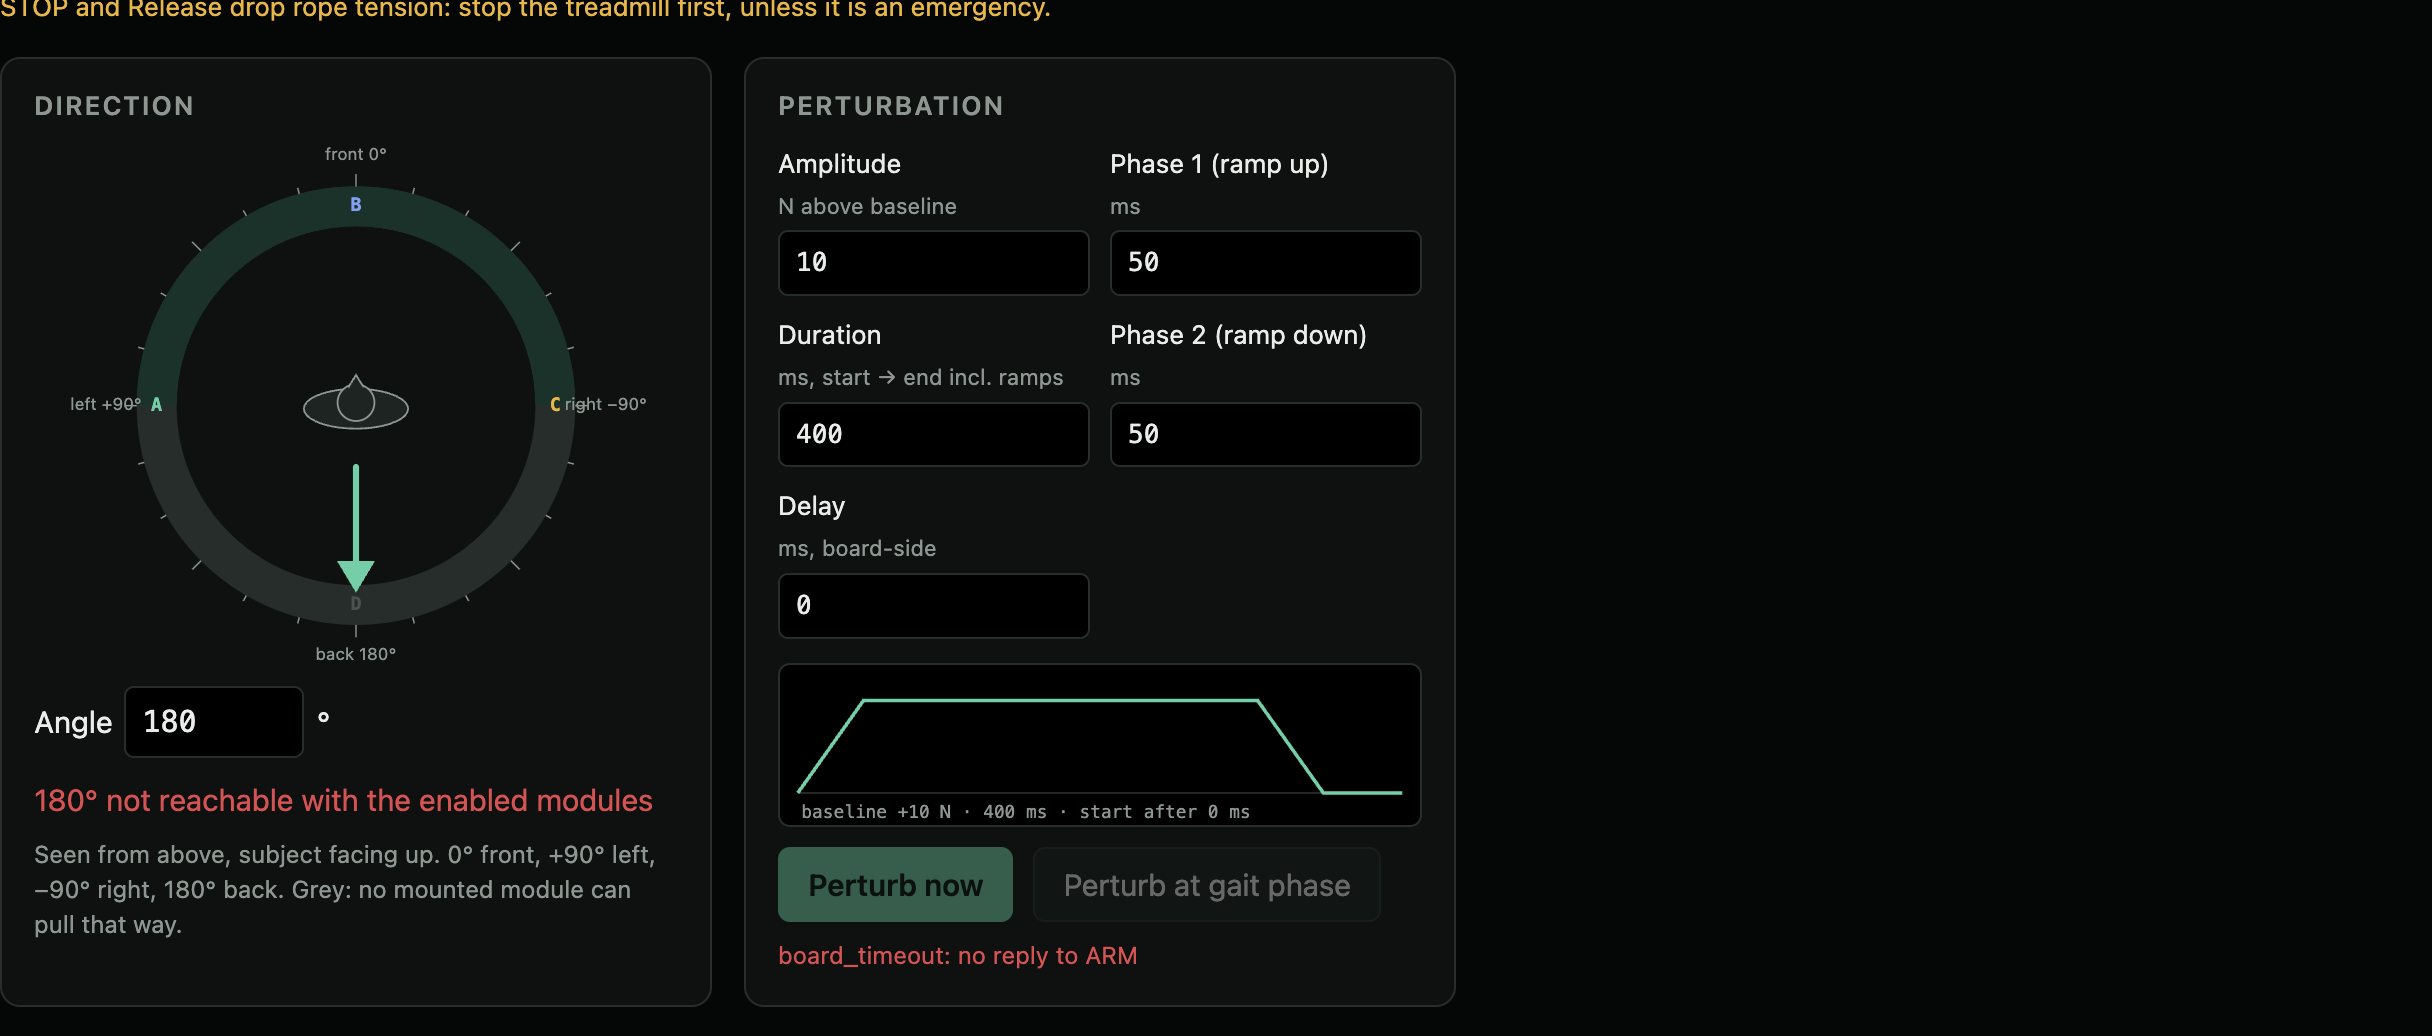
\includegraphics[width=\linewidth]{figures/ui-production.png}
\caption{Production page, 5 Oct 2026, B not installed so the front half of the dial is grey. The red
timeout under the button was the faulty USB socket, solved on 6 Oct.}
\end{figure}

\subsection{Not built yet}
\begin{enumerate}
\item \textbf{PTO}: perturb a set time or gait-cycle percentage after a foot strike (needs gait events,
first replayed, then from Vicon).
\item \textbf{Trials}: blocks, shuffled directions, 50--75 steps between perturbations, baseline from the
first 3\,s, logs. The schema is already proposed in \file{docs/API.md} (\cmd{planned}).
\item \textbf{Vicon live} on the lab PC (DataStream SDK) and the lab's balance-recovery algorithm
(\file{bumpem/recovery.py}, search \cmd{TODO(recovery)}).
\item Validate \file{bumpem/gait.py} against a recorded MATLAB log before live use.
\end{enumerate}

\subsection{How to change things}
\begin{itemize}
\item \textbf{New firmware behaviour}: \file{docs/PROTOCOL.md} first, then \file{firmware/src/main.ino},
then \file{bumpem/protocol.py} and \file{sim.py}. Re-flash.
\item \textbf{New endpoint}: \file{docs/API.md} first, then \file{server.py} + a test in
\file{tests/test_server.py}, then the UI.
\item \textbf{UI only}: edit \file{BumpemUI/web}, reload the page; test against \cmd{--board sim}.
\item After any change: \cmd{pytest}, update \file{docs/STATUS.md}, add a decision to
\file{docs/DECISIONS.md} if you chose between options, commit as \cmd{<area>: <what>}.
\end{itemize}
